\documentclass[prl,onecolumn,lengthcheck]{revtex4-2}

\usepackage{amssymb, amsmath, amsthm, amstext, amsfonts, amsopn, amscd}

\usepackage{color}
\usepackage{xcolor}
\usepackage[colorlinks=true, linkcolor=black, breaklinks=true, citecolor=blue, urlcolor=red]{hyperref} 
\usepackage{times}
\usepackage{mathdots}
\usepackage{graphicx}
\usepackage{tikz}
\usepackage{pgfplots}
\usetikzlibrary{decorations.markings}
\usetikzlibrary{decorations.pathreplacing,calligraphy}

%\usetikzlibrary{external}
%\tikzexternalize

\definecolor{spacecadet}{HTML}{0D284C}
\definecolor{munsell}{HTML}{008FA8}
\definecolor{banana}{HTML}{FFD932}
\definecolor{cgblue}{HTML}{007CA5}
\definecolor{isabelline}{HTML}{EAEDEA}

% The preamble here sets up a lot of new/revised commands and
% environments.  It's annoying, but please do *not* try to strip these
% out into a separate .sty file (which could lead to the loss of some
% information when we convert the file to other formats).  Instead, keep
% them in the preamble of your main LaTeX source file.


% The following parameters seem to provide a reasonable page setup.

%\topmargin 0.0cm
%\oddsidemargin 0.2cm
%\textwidth 16cm 
%\textheight 21cm
%\footskip 1.0cm


%The next command sets up an environment for the abstract to your paper.

%\newenvironment{sciabstract}{%
%\begin{quote} \bf}
%{\end{quote}}


\newcommand{\tr}{\operatorname{tr}}
\newcommand{\Tr}{\operatorname{Tr}}

\newcommand{\cA}{\mathcal A}\newcommand{\scrA}{\mathscr A}\newcommand{\fA}{\mathfrak A}
\newcommand{\ua}{\textup a}
\newcommand{\cB}{\mathcal B}\newcommand{\scrB}{\mathscr B}\newcommand{\fB}{\mathfrak B}
\newcommand{\C}{\mathbb{C}}
\newcommand{\cD}{\mathcal D}
\newcommand{\ud}{\textup d}
\newcommand{\cE}{\mathcal E}
\newcommand{\fF}{\mathfrak{F}}\newcommand{\cF}{\mathcal{F}}\newcommand{\sF}{\mathscr{F}}
\newcommand{\fg}{\mathfrak g}
\newcommand{\scrh}{\mathscr h}\newcommand{\fh}{\mathfrak h}
\newcommand{\cH}{\mathcal H}\newcommand{\fH}{\mathfrak H}\newcommand{\scrH}{\mathscr H}
\newcommand{\ltwo}{\ell^{2}}
\newcommand{\N}{\mathbb{N}}
\newcommand{\fP}{\mathfrak{P}}
\newcommand{\R}{\mathbb{R}}\newcommand{\cR}{\mathcal R}
\newcommand{\T}{\mathbb{T}}
\newcommand{\fu}{\mathfrak{u}}
\newcommand{\Z}{\mathbb{Z}}

\newcommand{\1}{\mathds{1}}

\newcommand{\vep}{\varepsilon}
\newcommand{\vth}{\vartheta}
\newcommand{\vp}{\varphi}


\begin{document} 

\title{Quantum Simulation of Conformal Field Theory} 

\author{Tobias J.\ Osborne$^{1}$ and Alexander Stottmeister$^{1}$}

\affiliation{$^{1}$Institut f\"ur Theoretische Physik, Leibniz Universit\"at Hannover, Appelstr. 2, 30167 Hannover, Germany}

\maketitle

\widetext

\begin{thebibliography}{61}%
\makeatletter
\providecommand \@ifxundefined [1]{%
 \@ifx{#1\undefined}
}%
\providecommand \@ifnum [1]{%
 \ifnum #1\expandafter \@firstoftwo
 \else \expandafter \@secondoftwo
 \fi
}%
\providecommand \@ifx [1]{%
 \ifx #1\expandafter \@firstoftwo
 \else \expandafter \@secondoftwo
 \fi
}%
\providecommand \natexlab [1]{#1}%
\providecommand \enquote  [1]{``#1''}%
\providecommand \bibnamefont  [1]{#1}%
\providecommand \bibfnamefont [1]{#1}%
\providecommand \citenamefont [1]{#1}%
\providecommand \href@noop [0]{\@secondoftwo}%
\providecommand \href [0]{\begingroup \@sanitize@url \@href}%
\providecommand \@href[1]{\@@startlink{#1}\@@href}%
\providecommand \@@href[1]{\endgroup#1\@@endlink}%
\providecommand \@sanitize@url [0]{\catcode `\\12\catcode `\$12\catcode
  `\&12\catcode `\#12\catcode `\^12\catcode `\_12\catcode `\%12\relax}%
\providecommand \@@startlink[1]{}%
\providecommand \@@endlink[0]{}%
\providecommand \url  [0]{\begingroup\@sanitize@url \@url }%
\providecommand \@url [1]{\endgroup\@href {#1}{\urlprefix }}%
\providecommand \urlprefix  [0]{URL }%
\providecommand \Eprint [0]{\href }%
\providecommand \doibase [0]{https://doi.org/}%
\providecommand \selectlanguage [0]{\@gobble}%
\providecommand \bibinfo  [0]{\@secondoftwo}%
\providecommand \bibfield  [0]{\@secondoftwo}%
\providecommand \translation [1]{[#1]}%
\providecommand \BibitemOpen [0]{}%
\providecommand \bibitemStop [0]{}%
\providecommand \bibitemNoStop [0]{.\EOS\space}%
\providecommand \EOS [0]{\spacefactor3000\relax}%
\providecommand \BibitemShut  [1]{\csname bibitem#1\endcsname}%
\let\auto@bib@innerbib\@empty
%</preamble>
\bibitem [{\citenamefont {Osborne}\ and\ \citenamefont
  {Stottmeister}(2021)}]{osborneConformal2021}%
  \BibitemOpen
  \bibfield  {author} {\bibinfo {author} {\bibfnamefont {T.~J.}\ \bibnamefont
  {Osborne}}\ and\ \bibinfo {author} {\bibfnamefont {A.}~\bibnamefont
  {Stottmeister}},\ }\bibfield  {title} {\bibinfo {title} {{Conformal field
  theory from lattice fermions}},\ }\bibfield  {journal} {\bibinfo  {journal}
  {arXiv: 2107.13834}\ }\href {https://doi.org/10.48550/arXiv.2107.13834}
  {10.48550/arXiv.2107.13834} (\bibinfo {year} {2021}),\ \Eprint
  {https://arxiv.org/abs/2107.13834} {2107.13834} \BibitemShut {NoStop}%
\end{thebibliography}%

%\newpage

\section{Supplementary material}

\begin{figure}[h]
	\begin{center}
	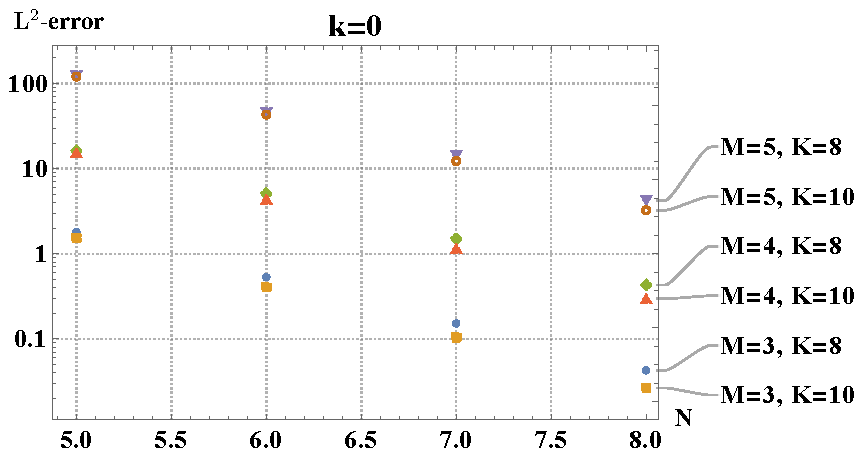
\includegraphics{figure3.pdf}
%	\begin{tikzpicture}
%	\draw (0,0) node{\includegraphics[width=0.9\textwidth]{plots/new/error_M345_k0.pdf}};
%	\draw (4.25,-3.15) node{\textbf{N}};
%	\draw (-6.35,3.6) node{$\mathbf{L}^{2}$-\textbf{error}};
%	\end{tikzpicture}
	\caption{Upper bound to the $L^{2}$-norm error between the conformal Hamiltonian $L_{0}$ and its KS approximant $L^{(N)}_{0}$ at $c=0$ on one-particle states corresponding to the subspace of the CFT Hilbert space representing wavelet details (for Daubechies wavelets D$K$) up to the simulation scale $M$ as a function of the UV cutoff scale $N$. For further details, see \cite{osborneConformal2021}.}\label{fig:waveleterrorM}
	\end{center}
\end{figure}

\begin{figure}[h]
	\begin{center}
	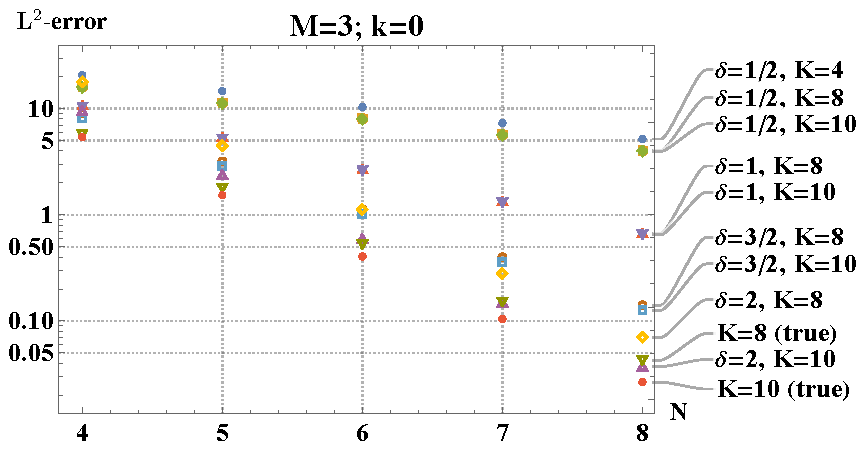
\includegraphics{figure4.pdf}
%	\begin{tikzpicture}
%	\draw (0,0) node{\includegraphics[width=0.9\textwidth]{plots/new/error_M3_k0.pdf}};
%	\draw (4.15,-3.1) node{\textbf{N}};
%	\draw (-6.3,3.55) node{$\mathbf{L}^{2}$-\textbf{error}};
%	\end{tikzpicture}
	\caption{Various upper bounds to the $L^{2}$-norm error between the conformal Hamiltonian $L_{0}$ and its KS approximant $L^{(N)}_{0}$ at $c=0$ on one-particle states corresponding to the subspace of the CFT Hilbert space representing wavelet details (for Daubechies wavelets D$K$) up to the simulation scale $M$ as a function of the UV cutoff scale $N$. The parameter $\delta$ is related to a factorized upper bound containing an $H^{\delta}$-Sobolev norm of the Daubechies D$K$ scaling function. For further details, see \cite{osborneConformal2021}.}\label{fig:waveleterrork}
	\end{center}
\end{figure}

\begin{figure}[h]
	\begin{center}
	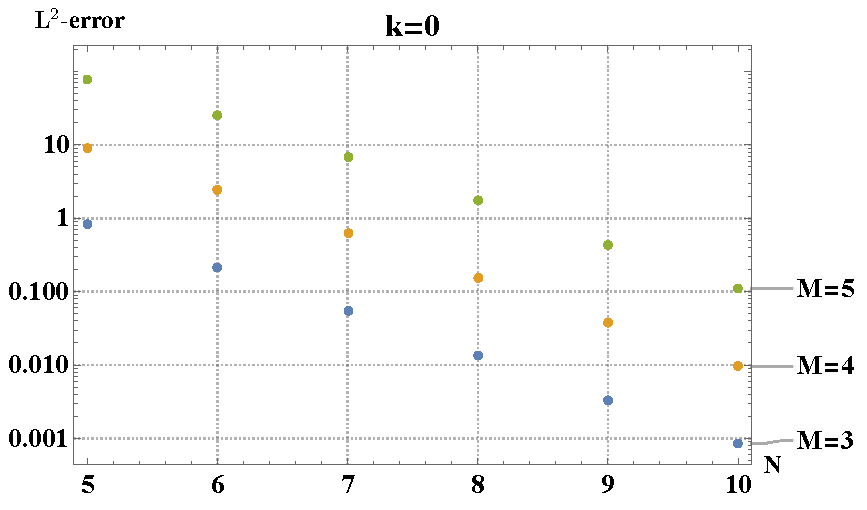
\includegraphics{figure5.pdf}
%	\begin{tikzpicture}
%	\draw (0,0) node{\includegraphics[width=0.9\textwidth]{plots/new/error_l2_mom-rg_M345.pdf}};
%	\draw (5.75,-3.55) node{\textbf{N}};
%	\draw (-6,4) node{$\mathbf{L}^{2}$-\textbf{error}};
%	\end{tikzpicture}
	\caption{Upper bound to the (diagonal) $L^{2}$-norm error between the conformal Hamiltonian $L_{0}$ and its KS approximant $L^{(N)}_{0}$ at $c=1/2,1$ on one-particle states corresponding to the subspace of the CFT Hilbert space representing momenta up to the simulation scale $M$ as a function of the UV cutoff scale $N$. For further details, see \cite{osborneConformal2021}.}\label{fig:momrgerrorM}
	\end{center}
\end{figure}

\begin{figure}[h]
	\begin{center}
	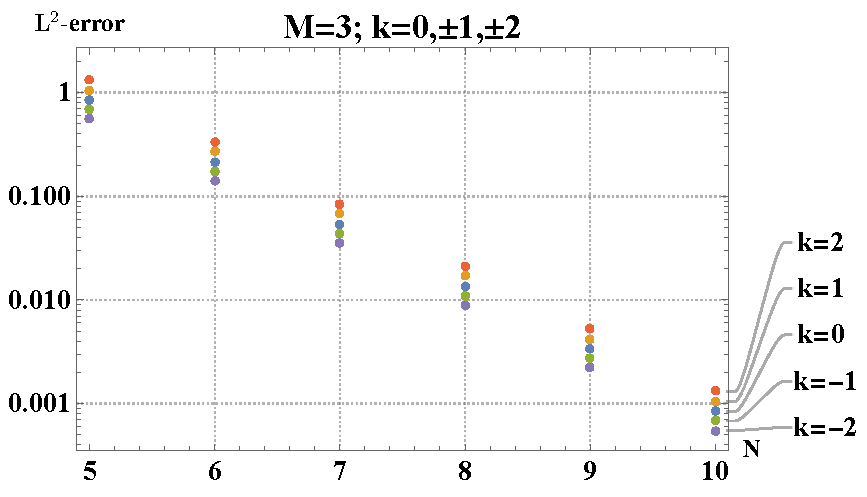
\includegraphics{figure6.pdf}
%	\begin{tikzpicture}
%	\draw (0,0) node{\includegraphics[width=0.9\textwidth]{plots/new/error_l2_mom-rg_M3_k012.pdf}};
%	\draw (5.4,-3.4) node{\textbf{N}};
%	\draw (-6,3.85) node{$\mathbf{L}^{2}$-\textbf{error}};
%	\end{tikzpicture}
	\caption{Upper bound to the (diagonal) $L^{2}$-norm error between the Virasoro generators $L_{k}$ and their KS approximants $L^{(N)}_{k}$ on one-particle states corresponding to the subspace of the CFT Hilbert space representing momenta up to the simulation scale $M$ as a function of the UV cutoff scale $N$. For further details, see \cite{osborneConformal2021}.}\label{fig:momrgerrork}
	\end{center}
\end{figure}

\begin{figure}[h]
	\begin{center}
	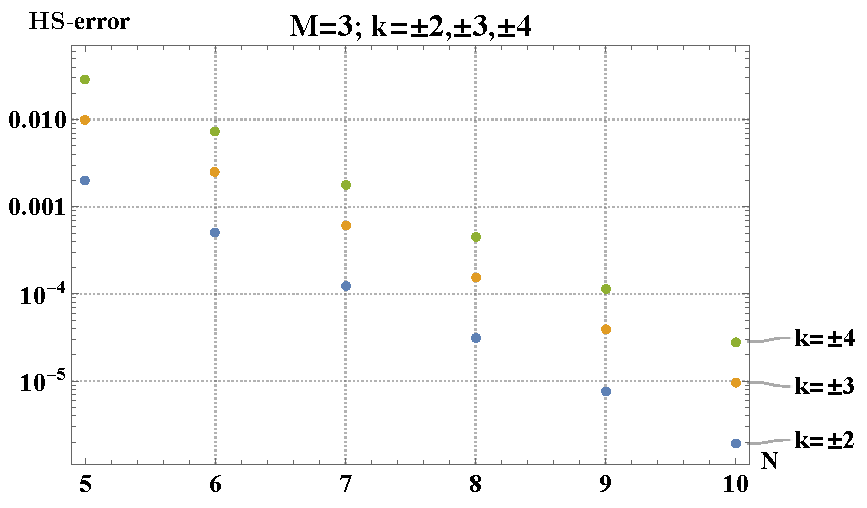
\includegraphics{figure7.pdf}
%	\begin{tikzpicture}
%	\draw (0,0) node{\includegraphics[width=0.9\textwidth]{plots/new/error_hs_mom-rg_M3_k234.pdf}};
%	\draw (5.7,-3.5) node{\textbf{N}};
%	\draw (-6,3.95) node{$\mathbf{HS}$-\textbf{error}};
%	\end{tikzpicture}
	\caption{Upper bound to the (off-diagonal) Hilbert-Schmidt (HS)-norm error between the Virasoro generators $L_{k}$ and their KS approximants $L^{(N)}_{k}$ on one-particle states corresponding to the subspace of the CFT Hilbert space representing momenta up to the simulation scale $M$ as a function of the UV cutoff scale $N$. Note, that this error vanishes for the generators of the Moebius group, $k=0,\pm 1$. For further details, see \cite{osborneConformal2021}.}\label{fig:momrgerrorHS}
	\end{center}
\end{figure}

\end{document}